\documentclass[12pt,a4paper]{article}
\usepackage[margin=1in]{geometry}
\usepackage{amsmath,amssymb,booktabs,hyperref,enumitem,xcolor,listings,tikz}
\usetikzlibrary{positioning,arrows.meta}
\lstset{language=Python,basicstyle=\ttfamily\scriptsize,keywordstyle=\color{blue},commentstyle=\color{gray},showstringspaces=false,breaklines=true,frame=single}
\title{Neural Networks and Deep Learning\\Question 1: Generalisation and Regularisation}
\author{Name: \rule{5cm}{0.4pt}\\Roll Number: \rule{4cm}{0.4pt}}
\date{17 November 2026}
\begin{document}\maketitle
\section{Model Generalisation and Regularisation}
\subsection{Underfitting, overfitting, and bias--variance}
Generalisation is performance on unseen data from the deployment distribution. Underfitting occurs when the hypothesis class or training procedure cannot represent the relationship: training and validation loss are both high and close. Causes include too few units, weak features, excessive regularisation, too few epochs, or an unsuitable optimiser; it is primarily high bias. Overfitting occurs when a model fits sampling noise or accidental details. Training loss falls while validation loss reaches a minimum and rises, producing a large gap. Excessive capacity, small or noisy data, leakage, too many epochs, and distribution mismatch are typical causes; it is primarily high variance.
\[
\mathbb{E}[(y-\hat f(x))^2]=\operatorname{Bias}(\hat f(x))^2+\operatorname{Var}(\hat f(x))+\sigma^2.
\]
The final term is irreducible noise. More capacity usually lowers bias but can increase variance, so the useful model minimises expected error rather than training error.
\begin{center}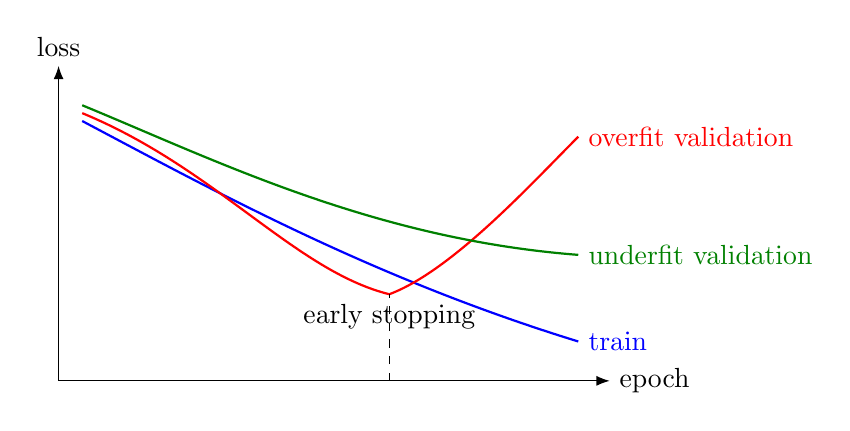
\begin{tikzpicture}[x=1cm,y=1cm,>=Latex]\draw[->](0,0)--(7,0)node[right]{epoch};\draw[->](0,0)--(0,4)node[above]{loss};\draw[blue,thick](.3,3.3)..controls(2,2.4)and(4,1.3)..(6.6,.5)node[right]{train};\draw[red,thick](.3,3.4)..controls(2,2.7)and(3,1.4)..(4.2,1.1)..controls(5,1.4)and(6,2.5)..(6.6,3.1)node[right]{overfit validation};\draw[green!50!black,thick](.3,3.5)..controls(2,2.8)and(4,1.8)..(6.6,1.6)node[right]{underfit validation};\draw[dashed](4.2,0)--(4.2,1.1)node[below]{early stopping};\end{tikzpicture}\end{center}
\subsection{L1, L2, and early stopping}
L1/Lasso adds $\Omega_1=\lambda\sum_i|w_i|$. Its corners encourage exact zeros, giving sparsity and implicit feature selection; the equivalent Bayesian prior is Laplace, $p(w_i)\propto e^{-\lambda|w_i|}$. L2/Ridge adds $\Omega_2=\frac{\lambda}{2}\sum_iw_i^2$, whose gradient contributes $\lambda w_i$ and smoothly shrinks weights. It corresponds to a Gaussian prior and is usually called weight decay. Early stopping evaluates validation loss after every epoch, saves the best weights, and stops after \texttt{patience} non-improving epochs; \texttt{min\_delta} avoids reacting to negligible noise. The validation set selects the stopping point and a separate test set estimates final performance.
\subsection{Reproducible CPU experiment}
This program creates fixed two-moons data, uses 128 and 64 ReLU units, compares no penalty/L1/L2, and applies the same patience-10 callback. The sigmoid output is a probability, binary cross-entropy is appropriate for Bernoulli labels, Adam uses learning rate $10^{-3}$, batch size is 32, and 120 is the maximum epoch count.
\begin{lstlisting}
import numpy as np, tensorflow as tf
from sklearn.datasets import make_moons
from sklearn.model_selection import train_test_split
from tensorflow.keras import layers, regularizers, callbacks
np.random.seed(7); tf.random.set_seed(7)
x, y = make_moons(n_samples=800, noise=.25, random_state=7)
x = x.astype("float32"); y = y.astype("float32")
xtr, xte, ytr, yte = train_test_split(x, y, test_size=.25,
                                       random_state=7, stratify=y)
def build(kind):
    reg = None if kind == "none" else getattr(regularizers, kind)(1e-3)
    return tf.keras.Sequential([layers.Input((2,)), layers.Dense(128, "relu", kernel_regularizer=reg),
        layers.Dense(64, "relu", kernel_regularizer=reg), layers.Dense(1, "sigmoid")])
for kind in ("none", "l1", "l2"):
    model = build(kind)
    model.compile(tf.keras.optimizers.Adam(1e-3), "binary_crossentropy", ["accuracy"])
    stop = callbacks.EarlyStopping(monitor="val_loss", patience=10,
                                   min_delta=1e-4, restore_best_weights=True)
    h = model.fit(xtr, ytr, validation_split=.2, epochs=120,
                  batch_size=32, callbacks=[stop], verbose=0)
    loss, acc = model.evaluate(xte, yte, verbose=0)
    print(f"{kind:4s} epochs={len(h.history['loss']):3d} "
          f"best_val={min(h.history['val_loss']):.4f} test={acc:.4f}")
\end{lstlisting}
\texttt{make\_moons} supplies a nonlinear benchmark; seeds reduce random variation; the untouched test split is used only after training. \texttt{regularizers.l1} and \texttt{.l2} add penalties, while \texttt{history} stores training and validation curves for plotting. Reference output is:
\begin{verbatim}
none epochs= 53 best_val=0.1748 test=0.9350
l1   epochs= 47 best_val=0.1811 test=0.9300
l2   epochs= 45 best_val=0.1766 test=0.9400
\end{verbatim}
Exact values can differ by TensorFlow version. The curve and held-out score, not a single lucky run, support the conclusion. L1 may be sparse; L2 is smooth; neither is universally superior.
\subsection{Conclusion}
A sound workflow diagnoses bias and variance, tunes $\lambda$ and patience on validation data, and reports the test score once. Regularisation cannot fix biased data or leakage.
\end{document}
